% !TEX root = main.tex
\section{Experiments and Results}
\label{sec:results}


\begin{table}[t]
    \begin{center}
    \setlength{\tabcolsep}{1.3mm}
\begin{tabular}{r|cccccccccc}
\hline
& PDIA  & PDIA-MAP &  HMM-EM & bigram& trigram & 4-gram & 5-gram & 6-gram & SSM \\
\hline
AIW & 5.13 & 5.46 &  7.89 & 9.71 & 6.45 & 5.13 & 4.80 & 4.69 & 4.78 \\
  & 365.6 & 379 & 52 & 28 & 382 & 2,023 & 5,592 & 10,838 & 19,358 \\
\hline
\hline
%AIWL & 4.08 & 4.13 &  7.89 & 9.45 & 5.72 & 4.05 & 3.51 & 3.32 & 3.24 \\
 %AIWL & 1,231.6 & 1,247 &  52 & 28 & 444 & 3,249 & 12,324 & 31,990 & 177,232 \\
%\hline
%\hline
DNA & 3.72 & 3.72 &  3.76 & 3.77 & 3.75 & 3.74 & 3.73 & 3.72 & 3.56 \\
 & 64.7 & 54 & 19 &  5 & 21 & 85 & 341 & 1,365 & 314,166 \\
\hline
\end{tabular}
\end{center}
\caption[Short]{PDIA inference performance relative to HMM and fixed order Markov models.  Top rows: perplexity.  Bottom rows: number of states in each model.  For the PDIA this is an average number.\label{table:results}}
\end{table}
%
To test our PDIA inference approach we evaluated it on discrete natural sequence prediction and compared its performance to HMMs and smoothed $n$-gram models.  We trained the models on two datasets: a character sequence from {\em Alice in Wonderland} \cite{Carroll1865} and a short sequence of mouse DNA.  The {\em Alice in Wonderland} (AIW) dataset was preprocessed to remove all characters but letters and spaces, shift all letters from upper to lower case, and split along sentence dividers to yield a 27-character alphabet (a-z and space)\comment{ and 1,639 sentences with a total of 132,794 characters.  We used the first 1,200 sentences (100,210 characters) to train the models and the rest to test}.  We trained on 100 random sentences (9,986 characters) and tested on 50 random sentences (3,891 characters).   The mouse DNA dataset consisted of a fragment of chromosome 2 with 194,173 base pairs, which we treated as a single unbroken string.  We used the first 150,000 base pairs for training and the rest for testing.  For AIW, the state of the PDIA model was always set to $q_0$ at the start of each sentence.  For DNA, the state of the PDIA model at the start of the test data was set to the last state of the model after accepting the training data.  We placed Gamma(1,1) priors over $\alpha$, $\beta$ and $\gamma$ and set $\lambda=.001$.

We evaluated the performance of the learned models by calculating the average per character predictive perplexity of the test data.  For training data $x_{1:T}$ and test data $y_{1:T'}$ this is given by $2^{-\frac{1}{T'}\log_2\, P(y_{1:T'}|x_{1:T})}$.  It is a measure of the average uncertainty the model has about what character comes next given the sequence up to that point, and is at most $|\Sigma|$.  We evaluated the probability of the test data incrementally, integrating the test data into the model in the standard Bayesian way\comment{, and averaged each predictive probability $P(y_{1:T'}|x_{1:T}) =  \prod_{i = 1}^{T'} \int P(y_i|y_{1:i-1},x_{1:T},\delta)P(\delta|y_{1:i-1},x_{1:T})d\delta \approx \frac{1}{L}\prod_{i = 1}^{T'} \sum_{\ell = 1}^{L} P(y_i|y_{1:i-1},x_{1:T},\delta_\ell)$ where $\delta_\ell \sim P(\delta|y_{1:i-1},x_{1:T})$}.  



Test perplexity results are shown in Table~\ref{table:results} on the first line of each subtable.  Every fifth sample for AIW and every tenth sample for DNA after burn-in was used for prediction.  For AIW, we ran 15,000 burn-in samples and used 3,500 samples for predictive inference.  Subsampled sampler diagnostic plots are shown in Figure~\ref{fig:aiw_sampler_trace} that demonstrate the convergence properties of our sampler.  When modeling the DNA dataset we burn-in for 1,000 samples and use 900 samples for inference.
For the smoothed $n$-gram models, we report thousand-sample average perplexity results for hierarchical Pitman-Yor process (HPYP) \cite{Teh2006a} models of varying Markov order (1 through 5 notated as bigram through 6-gram) after burning each model in for one hundred samples.  We also show the performance of the single particle incremental variant of the sequence memoizer (SM) \cite{Gasthaus2010}, the SM being the limit of an $n$-gram model as $n\rightarrow\infty$.
We also show results for a hidden Markov model (HMM) \cite{Murphy2005} trained using expectation-maximization (EM).  We determined the best number of hidden states by cross-validation on the test data (a procedure used here to produce optimistic HMM performance for comparison purposes only).  

%The log loss and optimal number of states are given in Table \ref{table:results}, and plots showing the generalization performance across a range of model sizes relative to PDIA performance is given in Figures \ref{fig:dna_hmm} and \ref{fig:aiw_small_hmm}.  

The performance of the PDIA exceeds that of the HMM and is approximately equal to that of a smoothed 4-gram model, though it does not outperform very deep, smoothed Markov models \comment{(the performance of the SSM on AIW is likely due to the incremental and single-particle approach to prediction)}.  This is in contrast to \cite{Thollard2001}, which found that PDFAs trained on natural language data were able to predict as well as {\em unsmoothed} trigrams, but were significantly worse than smoothed trigrams, even when averaging over multiple learned PDFAs.  As can be seen in the second line of each subtable in Table~\ref{table:results}, the MAP number of states learned by the PDIA is significantly lower than that of the $n$-gram model with equal predictive performance.

Unlike the HMM, the computational complexity of PDFA prediction does not depend on the number of states in the model because only a single path through the states is followed.  This means that the asymptotic cost of prediction for the PDIA is $\mathcal{O}(LT')$, where $L$ is the number of posterior samples and $T'$ is the length of the test sequence.  For any single HMM it is $\mathcal{O}(KT')$, where $K$ is the number of states in the HMM.  This is because to achieve the given HMM predictive inference performance all possible paths must be followed (although theoretically fewer than K could be followed if doing approximate inference).  In PDIA inference we too can choose the number of samples used for prediction, but here even a single sample has empirical prediction performance superior to averaging over all paths in an HMM.  The computational complexity of smoothing $n$-gram inference is equivalent to PDIA inference, however, the storage cost for the large $n$-gram models is significantly higher than that of the estimated PDIA for the same predictive performance.%In addition to averaging over multiple $\delta_\ell$, we also evaluated the log loss for each $\delta_\ell$ by itself to find the single model with the best generalization performance, which we call $\delta_{MAP}$.

%Note that we could have compared PDIA inference performance to an HDP-HMM model \cite{Teh2006b} but chose not to for two reasons.  First, averaging over multiple PDFAs is roughly comparable computationally to inference in a single HMM, whereas HDP-HMM inference is significantly more costly.  Second, on data similar but smaller than that used here, the HDP-HMM did not significantly outperform the best EM-trained HMM \cite{Teh2006b}.

\comment{The predictive performance relative to the HPYP $n$-gram is particularly unexpected given that there is no smoothing hierarchy over the states in the PDIA.  In an $n$-gram model, each state is identified with a context, and thus a natural hierarchy exists for smoothing states by more general states.  In the PDIA states are not identifiable and no hierarchy on which smoothing can be implemented is apparent.  Instead, the PDIA improves predictive performance by averaging over model structure.  Because these models are simple, averaging over structure is computationally feasible, and makes practical an underexplored approach to smoothing.}

\comment{While the PDIA averages over a  class of models that includes finite order Markov models as a subset, the states in HPYP are identifiable which means that hierarchical smoothing of the per-state emission distributions is possible.  In the PDIA model the states are not identifiable and no easily defined hierarchy of contextual specificity exists on which hierarchical smoothing can be implemented.   Note that the PDIA posterior average achieves}


\begin{figure}[htbp]
\centering
%\subfigure[DNA HMM EM Baseline]{\label{fig:dna_hmm}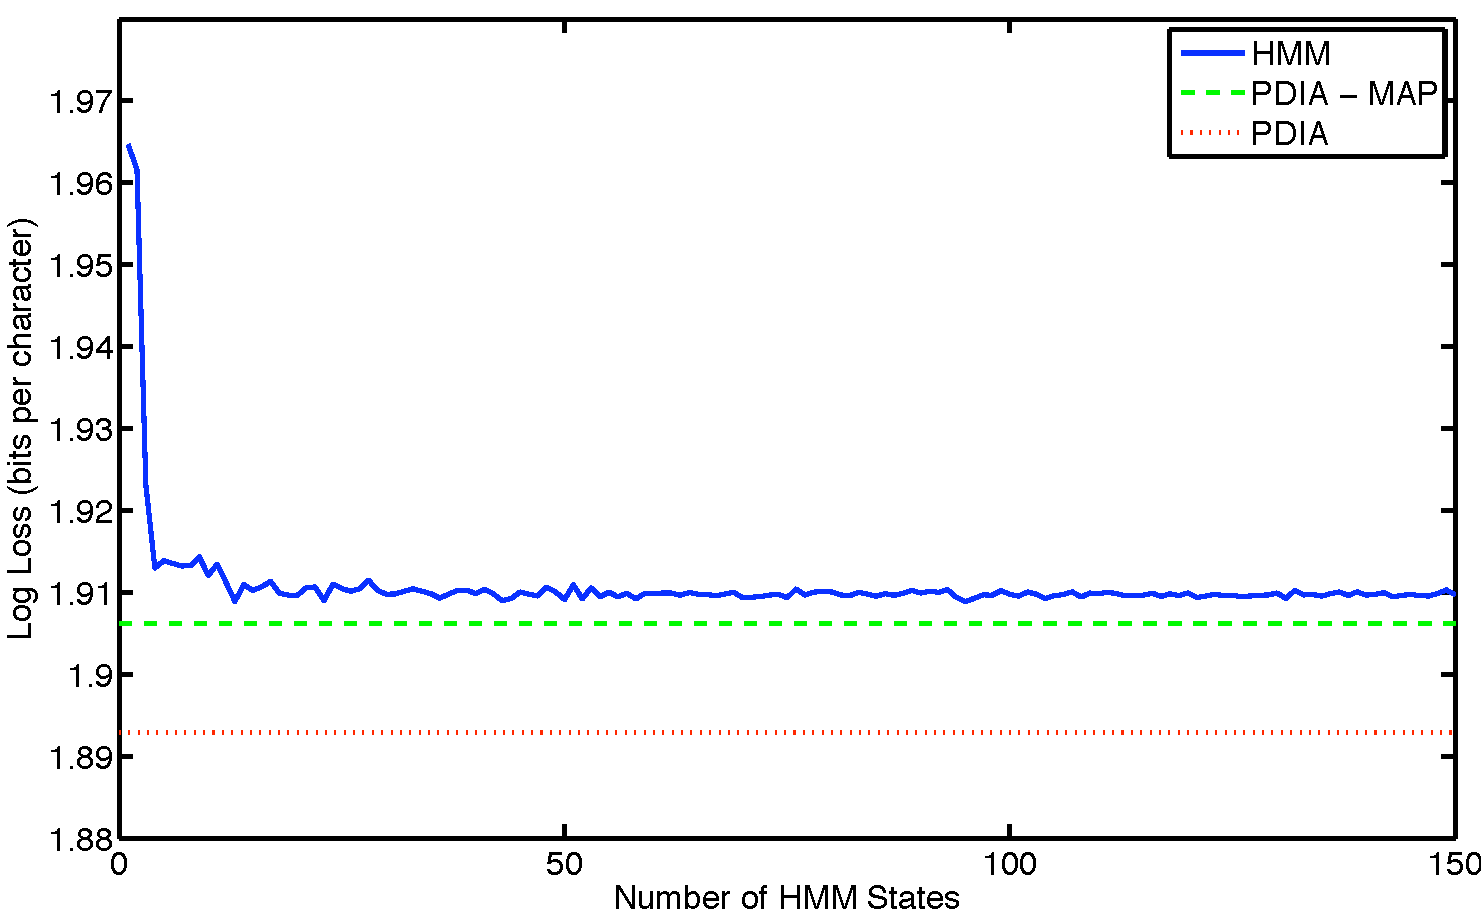
\includegraphics[width=.3\textwidth]{results/dna_hmm}}
%\subfigure[DNA]{\label{fig:dna_sampler}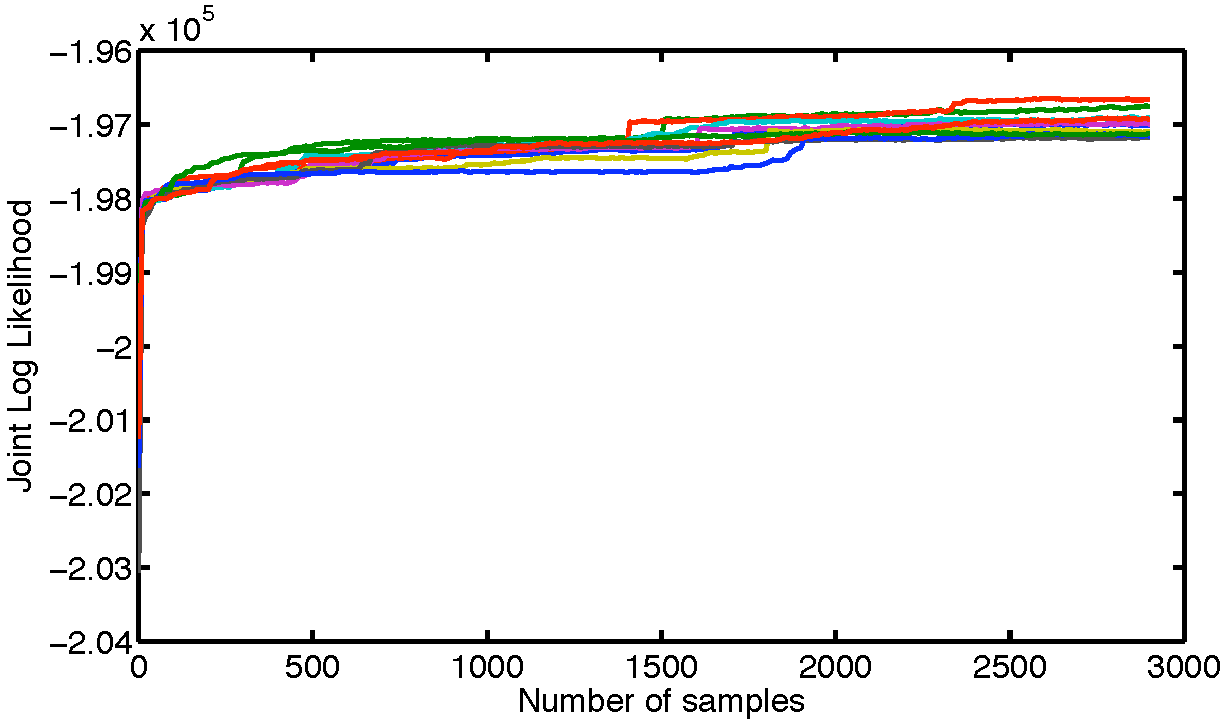
\includegraphics[width=.3\textwidth]{results/dna_sampler}}
%\subfigure[DNA number of states]{\label{fig:dna_numstates}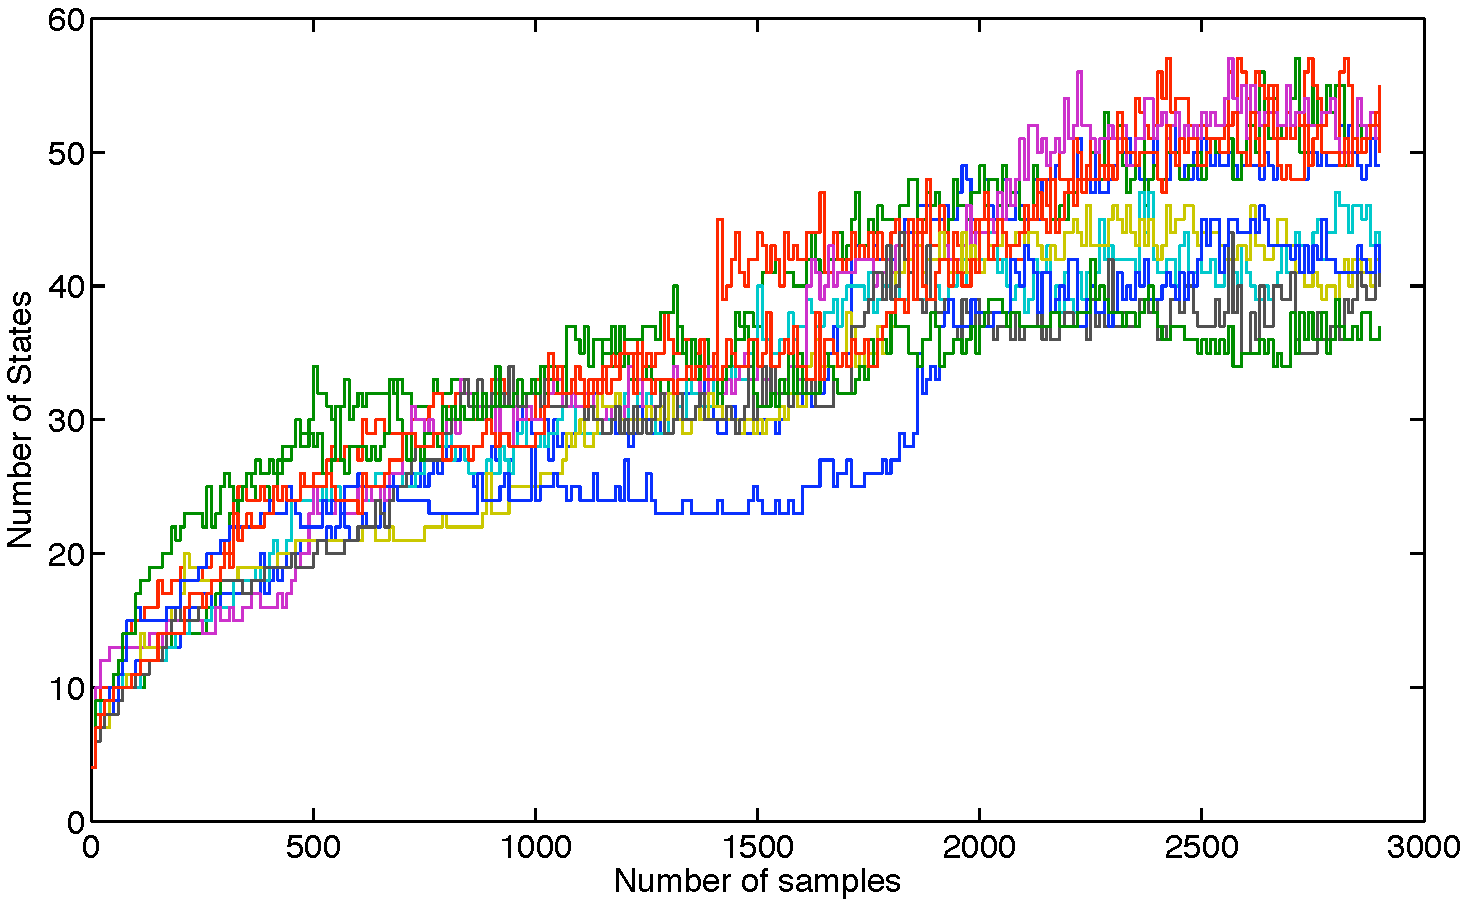
\includegraphics[width=.3\textwidth]{results/dna_numstates}}\\
%\subfigure[AIW HMM Baseline]{\label{fig:aiw_hmm_baseline}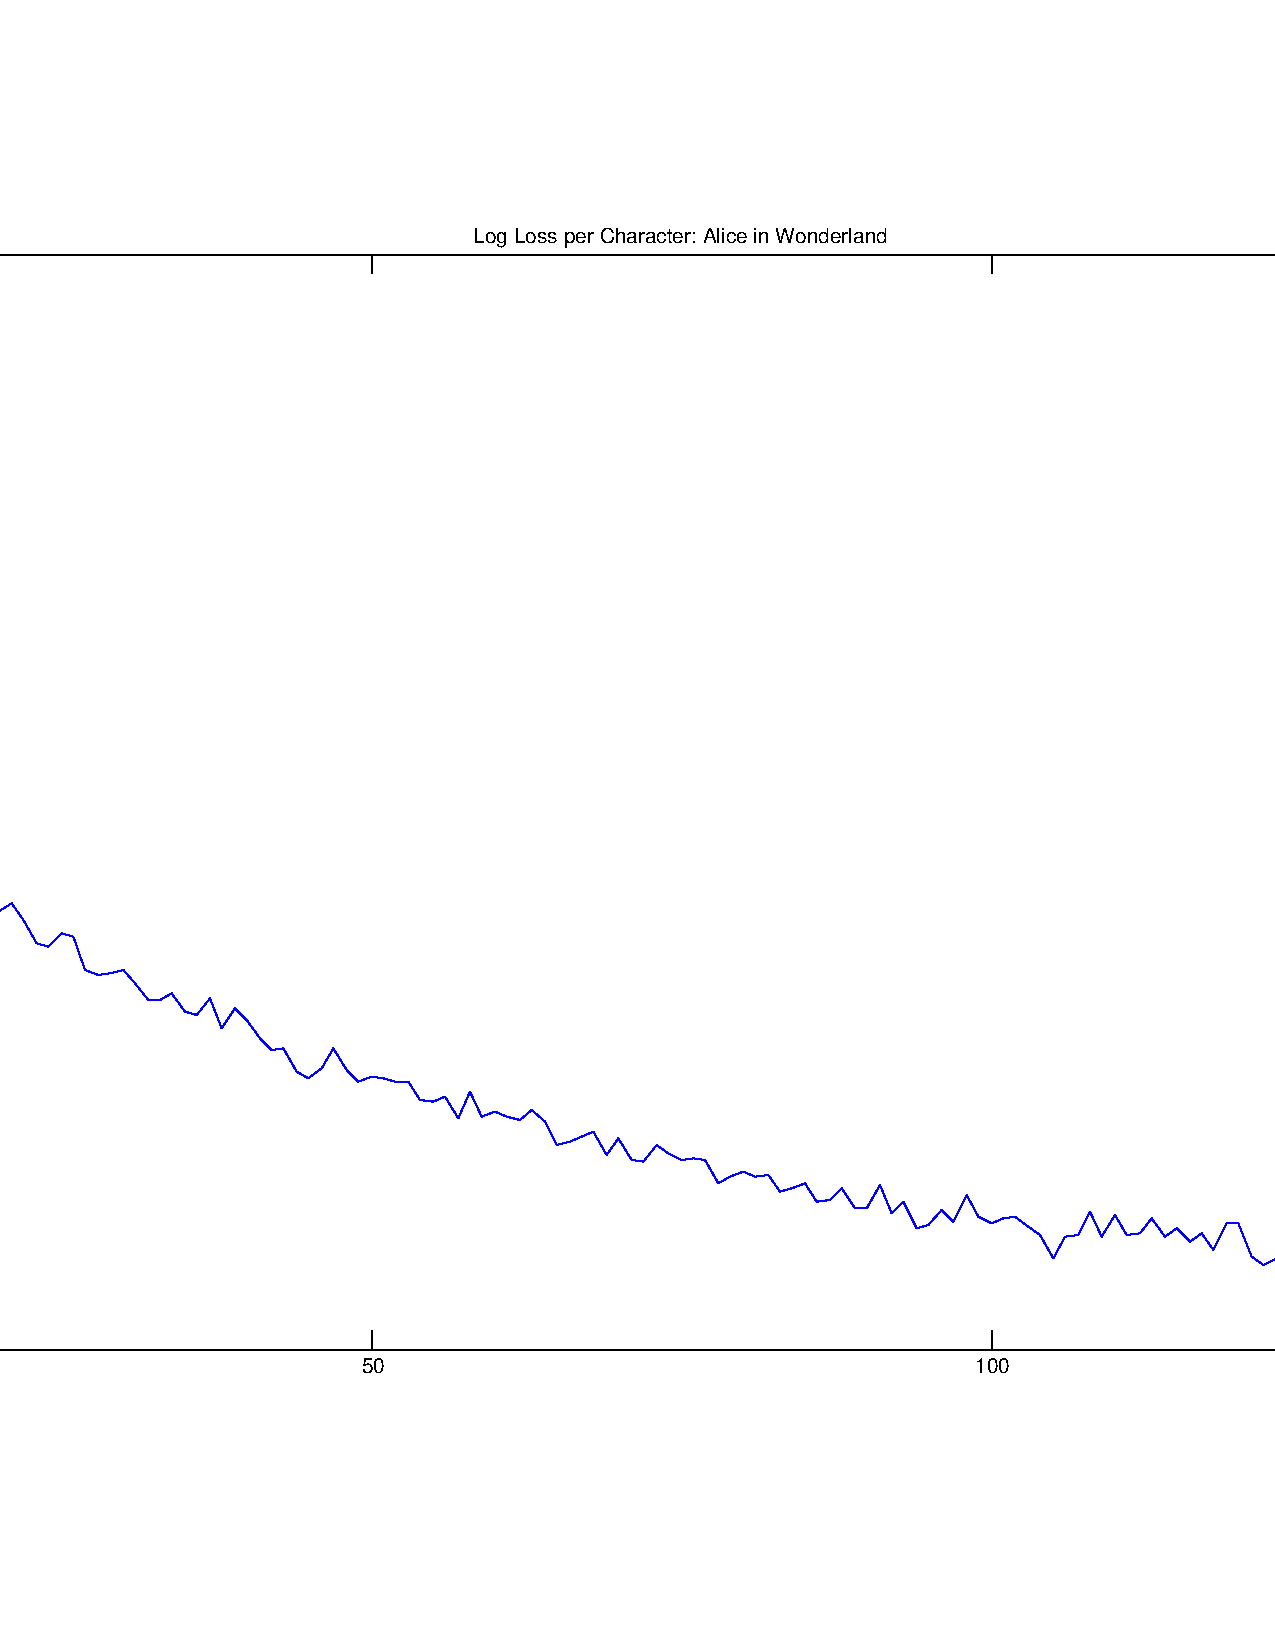
\includegraphics[width=.45\textwidth]{results/aiw_hmm_baseline}}
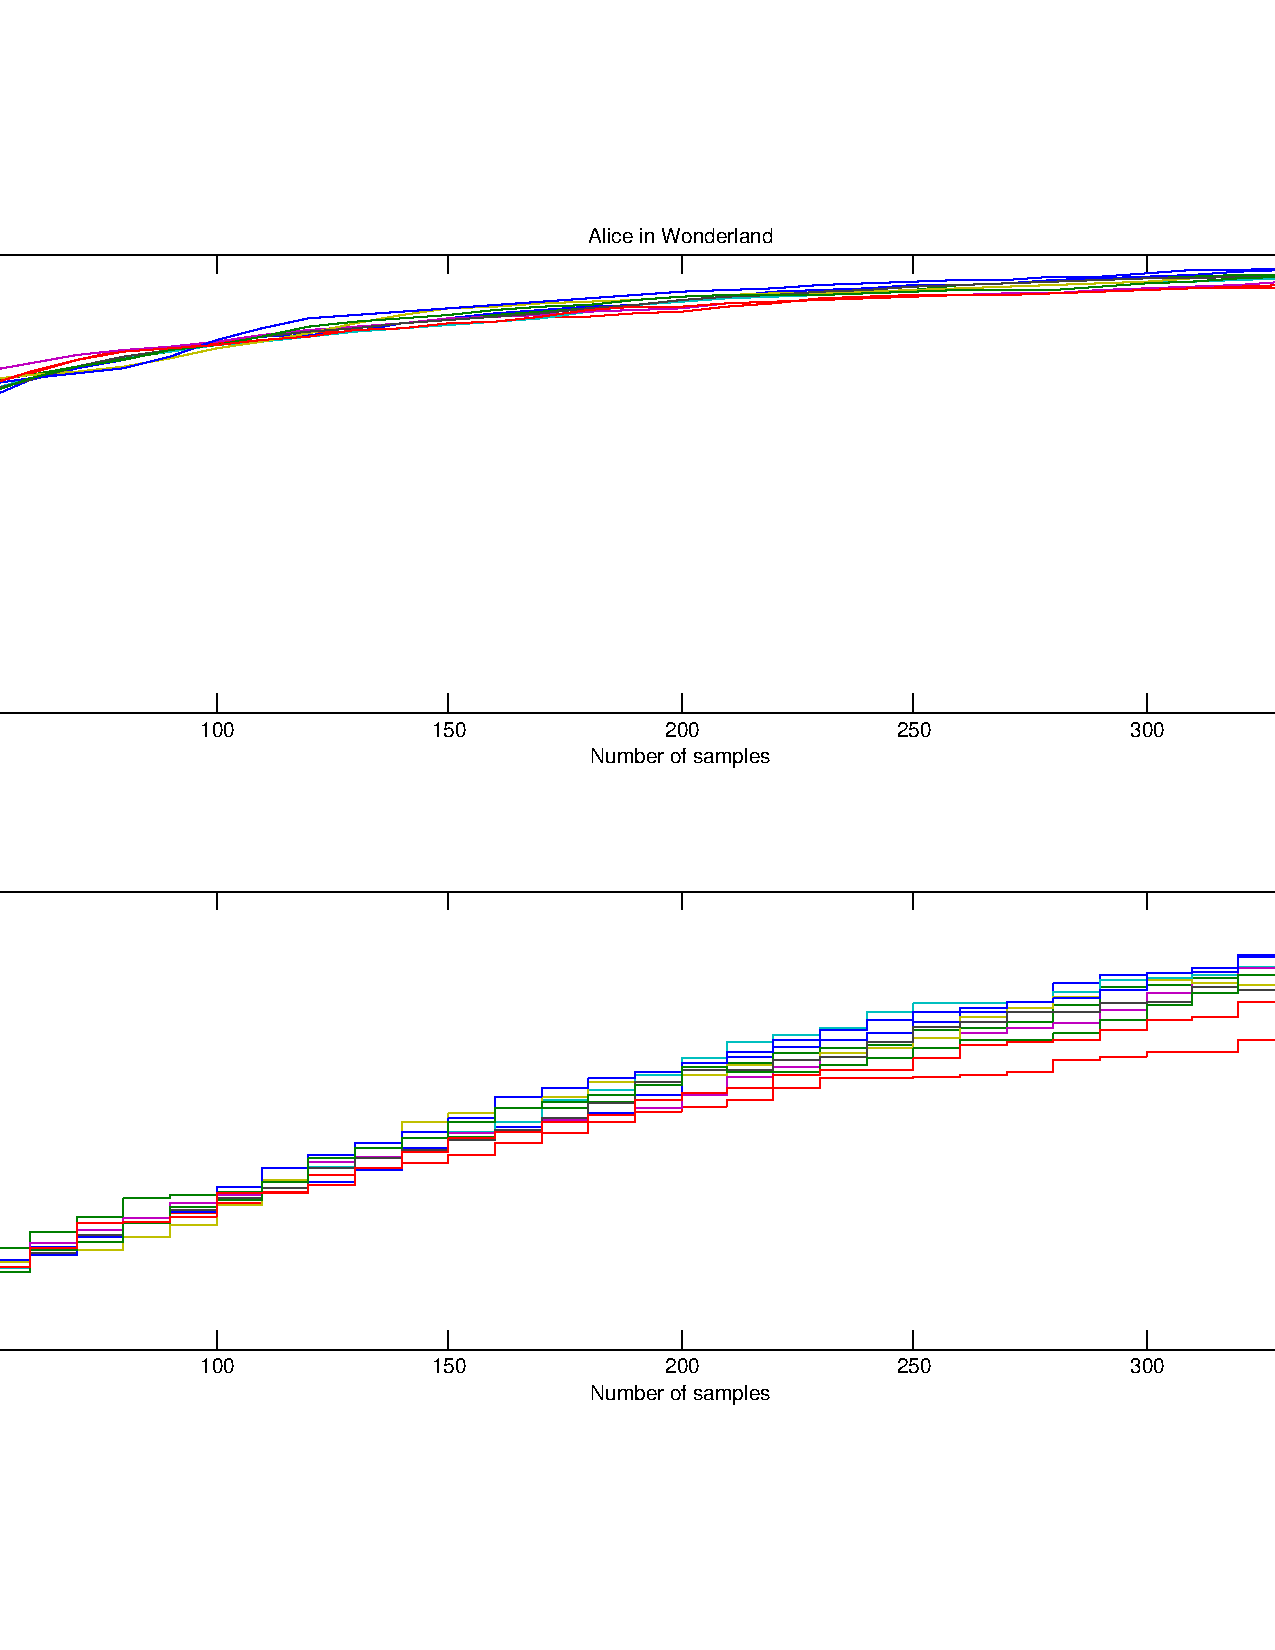
\includegraphics[width=1\textwidth]{results/aiw_sampler_trace}
%\subfigure[AIW number of states]{\label{fig:aiw_small_numstates}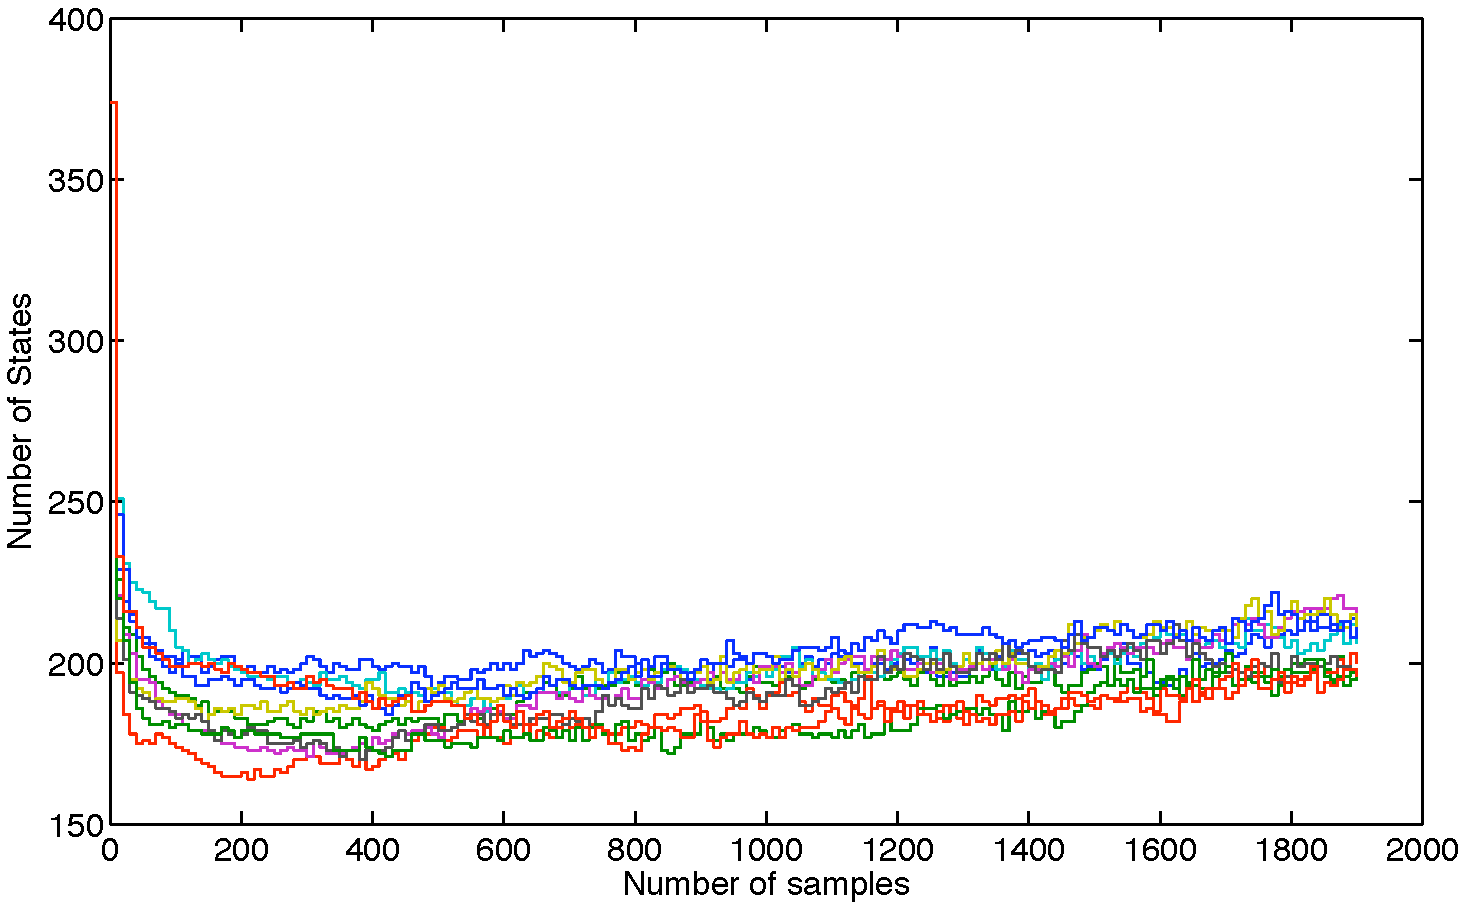
\includegraphics[width=.3\textwidth]{results/aiw_small_numstates}}
\caption{PDIA sampler trace for Alice in Wonderland.  The top trace is the joint log likelihood of the model and training data, the bottom trace is the number of states.\label{fig:aiw_sampler_trace}}
\end{figure}





%We found that both the MAP PDIA and the average over PDIA generalize better than the HMM.  To test the possibility that better generalization was due to smoothing of the PDIA emission probability by $\beta$, we took samples from the PDIA, fixed $\beta$ to be very near 0, and ran the MCMC sampler as before.  We found that neither the average number of states nor the generalization performance was significantly affected.

%In general it seems that posterior samples from the PDIA achieve competitive generalization performance on natural language and DNA compared to hidden Markov models and n-gram models.  Averaging predictive probability over multiple samples leads to better generalization than a single sampled model.  Both a single sample and multiple samples generalize better than the best EM-trained HMM.  On natural language, the learned PDIA has more states than the optimal number of states for an HMM found by cross-validation.  The improved generalization is not due to smoothing the emission distribution.  Compared to smoothed n-gram models, the PDIA performs competitively even though there is no backing off to more general contexts.




%Even for a single sampled transition matrix $\delta_\ell$, there may be symbols $y_t$ which have not been emitted from the state $\q_t$ in the training data, and thus $\delta_\ell(\q_t,y_t)$ is not known.  In this case we sampled a new element of the transition matrix according to the CRF, as described in \ref{model}.  In the same way that we averaged the predictive probability of each character over multiple $\delta_\ell$, we averaged the probability of a character given a single $\delta_\ell$ over multiple sampled values of $\delta_\ell(\q_t,y_t)$.



